\chapter{绪论}
\label{chap01}
近年来,随着互联网技术的发展,在线社交网络(Online Social Networks)在全世界范围内普及开来,其应用融入到了人们生活的方方面面之中。近十年来,对于在线社交网络的研究一直持续增长。在很大程度上,这归功于社交媒体以及社交服务网站的蓬勃发展。这些媒体以及网站的迅猛发展给社交网络分析(Social Network Analysis)提供了丰富的语料库与数据集。而对社交网络的研究与应用也促进了社交媒体以及社交服务网站的持续发展。在线社交网络是社会中个体集合以及个体之间连接关系所构成的网络在网络空间上的映射,即在线社交网络是真实社会在虚拟网络中的体现和拓展。在线社交网络加速了拉近了人与人之间的距离,加快了信息传播的速率,丰富了群体的结构关系。因此,在线社交网络成为了社会学、传播学、计算机科学以及系统科学等领域的研究热点。

在线社交网络是在信息网络上由用户集合以及用户之间关系所构成的社会性结构,一般而言包含三个要素:“关系结构”、“网络群体”以及“网络信息”\upcite{方滨兴2014在线社交网络分析}。三个要素之间相互关联、相互依存,其关系如图\ref{fig:threeFactors}所示。其中关系结构为网络群体的互动行为提供了基础结构以及底层平台,是社交网络的载体;网络群体推动网络信息传播,影响关系结构的演化,是社交网络的主体;网络信息的内容和传播是社交网络关键点,是群体行为的诱因和效果,同时也影响关系结构的变化,是社交网络的客体。

\begin{figure}[!ht]
    \centering
    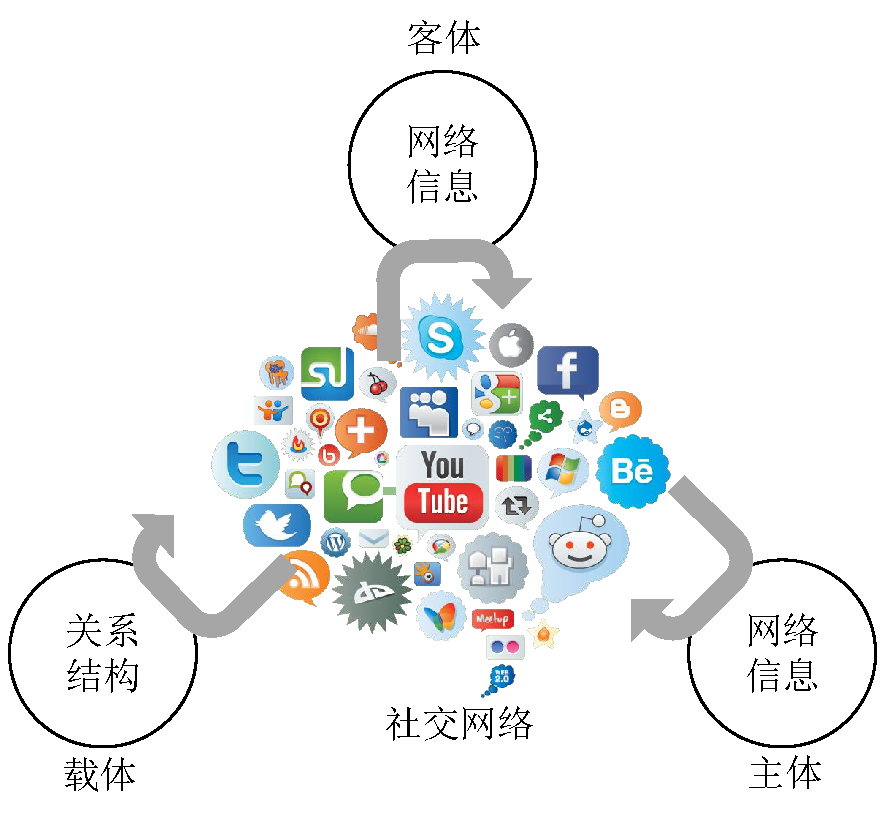
\includegraphics[width=0.5\textwidth]{threeFactors}
    \caption{在线社交网络中的关系结构、网络群体和网络信息}
    \label{fig:threeFactors}
\end{figure}

与传统的Web应用和信息媒体相比,在线社交网络具有如下的新特性:
\begin{itemize}
	\item 高速性:信息发布和接收十分便捷、迅速。社交网络中的用户可以通过手机、笔记本电脑等终端随时随地发布和接收信息,信息传递的效率高,具有高速性。
	\item 扩散性:裂变式的信息传播。社交网络中的信息一经发布,便会立刻推送到所有的关注者。信息经过转发,信息又将传播到下一批关注者。信息的传播呈现一种链式反应的几何级数扩散模式,为普通网民传播信息提供了渠道。
	\item 平等性:人人都有可能成为信息输出者。与传统信息媒体中信息发布和信息接收的非对称性相比,社交网络中的每一个参与者都有机会通过社交网络表达自己的观点,传播自己的信息,输出自身的价值观。因此,社交网络在热点事件的产生、发酵、传播等环节中扮演了重要的角色。
	\item 自发性:呈现自媒体形态、自发地形成虚拟社区。社交网络中的个体既是信息的接收者也是信息的发布者,用户会根据自身不同的关注内容与其他用户建立联系,形成网络中的虚拟社区。
\end{itemize}

这些丰富的特性让在线社交网络具有和其他信息媒体不一样的特点,同时也对信息安全提出了新的挑战。对于社交网络分析的研究,在结构、群体以及信息等方面都存在很多已有的工作。其中很多研究工作是关于网络中的信息传播、影响力、传播模型等。这些工作主要研究是否可以建立模型来解释信息的传播方式,如何在真实社交网络信息传播数据集上验证传播模型等等,这些仅仅是社交网络中信息传播研究的一些研究举例。信息传播在实际生活中有着许多应用,例如商业产品或者理念的病毒式营销、网络流量的爆发检测、寻找关键博客来获取重要的信息、寻找意见领袖或者潮流带动者以及信息的检索排序等等。

社交网络中信息传播关键技术的研究对于理解信息传播的机理有着重要的意义。本文首先在结构上进行理论研究,思考在社交网络中如何选取源节点才能使得信息传播效率更高,提出了传播效率最大化问题。然后,本文在内容方面进行分析,利用语言模型以及深度学习等技术,对普通文本信息以及数据流信息进行应用,进行了基于语义扩展和文本质量的实时个性化搜索研究和基于卷积神经网络的文本分类研究,分析不同用户的关注点,将用户所感兴趣的、高质量的信息自动地推送给用户,使得用户更加便捷地获取信息,从而推动信息的传播。最后,本文建立传播模型,对于事件的传播影响进行评估,来估测事件传播影响面的大小。本研究对于揭示信息传播的机理和规律、推动社交网络中的信息传播、发现有价值的信息以及保护信息安全起到了重要的作用。

本章首先对本文的研究背景进行阐述,第\ref{sec1:background}小节对在线社交网络中信息传播研究的发展现状进行描述,分析社交网络信息传播分析的研究意义和面临的挑战。其次,第\ref{sec1:relatedWorks}小节对本文研究的各个相关工作进行了概述和总结。然后,第\ref{sec1:inovation}小节介绍本文的主要研究内容和创新点。最后,第\ref{sec1:paperStructure}小节给出了本文的组织结构。

\section{研究背景及意义}
\label{sec1:background}
本节主要介绍本文研究的背景及其意义,对涉及到的概念进行详细的阐述,对研究所面临的挑战进行分析。首先,本节对在线社交网络进行一个概述,介绍在线社交网络的起源、定义、特点以及发展状况。其次,本节对社交网络中的信息传播进行介绍,详细地描述信息传播的特点及其所涉及到的因素。然后,本节对本文的研究的意义进行总结。最后,本节分析了研究所面临的挑战。
\subsection{在线社交网络概述}
\label{subsec1:introduction}
从人类诞生以来,就过着群居的生活,一同劳作、交流以及分享,从而形成了社会。随着人类文明的发展和社会的进步,人与人之间的关系进一步的深入和加强,社会关系由简单的血缘关系向朋友关系、雇佣关系以及社交关系发展。而人与人之间由生活、工作、学习、娱乐等等社会交互而形成了某种稳定的关系,这一系列的关系将社会个体结合成了一个巨大的网络,这即是社交网络。如同Linton Freeman所说的那样,我们都被一个无形的网络连接在一起\upcite{freeman2004development}。

社交网络(Social Network)在维基百科中被定义为由社会个体(例如个人或者机构等)、社会个体间的二元关系以及社会个体之间的社交互动组成的社会结构\upcite{social_network}。在社交网络中,个体之间因为社交互动而形成相对稳定的关系体系,这种关系可能是亲属关系、朋友关系、同学关系,也可能是商业合作关系或者宗教信仰关系等。通过这些关系,社交网络把偶然相识的弱关系到紧密结合的强关系,以及社会中各式各样的人群串联成了一张巨大的网络。由于社交网络中存在这各种各样的社会关系,个体之间的网络结构往往是非常复杂的。而且,复杂的关系结构也会影响网络中个体之间的社交互动,进而影响到个体的社会行为。

随着工业化、城市化的进行以及移动网络的发展,社会网络化的趋势日益凸显。在2012年,Lee Rainie和Barry Wellman在其著作《网络化:新的社会操作系统》\upcite{rainie2012networked}中指出,社会网络革命、移动革命以及互联网革命将是影响人类社会发展的三大革命。随着互联网的进步,网络结构受地域性因素的影响减弱了,这使得跨地域性的线上社会关系成为了社交网络的主要形式。在现实社会中,人们相继在社交媒体平台上创建账号,将线下的社会关系扩展到了线上,并且进行了进一步的延伸,这使得在线社交网络成为了人们网络生活中不可或缺的沟通工具。

在2009年欧盟关于社会计算的研究报告中\upcite{huijboom2009key},在线社交网络主要可以分成如下的四个大类,
\begin{itemize}
	\item 即时通讯应用。这一类的应用提供一个实时的通信平台,使得人与人之间能够通过网络进行在线的交流,信息的分享等。典型的代表有MSN、QQ、飞信等,其具有双向认证与实时推送的特点。
	\item 在线社交应用。这一类的应用提供一个在线社交关系平台,人们在平台上进行社交互动以及消息的共享等。典型的代表有脸书(Facebook)、谷歌+(Google+)、人人网、QQ空间等,其具有双向认证以及非实时推送的特点。
	\item 微博类型应用。这一类的应用提供一个自媒体的信息发布平台,任何个人或者机构都能在平台上发布信息,推送给其关注者。典型的代表有推特(Twitter)、新浪微博、腾讯微博等,其具有单向认证以及实时推送的特点。
	\item 共享空间以及其他应用。这一类的应用提供一个公告发布系统,具有沟通功能,但是用户之间结合不紧密。典型的代表有BBS、论坛、博客等,其具有单向认证以及非实时推送的特点。
\end{itemize}

社交网络是Web 2.0时代的具有代表性的应用,具备Web 2.0时代交互性、主动性的特点,众多社交软件应用随着技术的更新而蓬勃发展。中国流行的即时通信软件“腾讯QQ”诞生于1999年,在2016年的月活跃账户数(MAU)达到8.77亿,其中智能终端月活跃账户达到6.47亿\upcite{tencentReport2016}。2004年于美国上线的社交网络服务网站脸书(Facebook)成为了全球范围内最流行的社交网站之一。从网站成立至今,其用户持续增长,在2016年第四季度,脸书月活跃人数已经突破了18.6亿,其中移动端用户数达到了17.4亿\upcite{facebookReport2016}。2006年微博客类的应用推特(Twitter)在美国诞生,允许用户更新不超过140个字符的消息,成为一个广受欢迎的社交网络及微博客服务网站。截至2016年第四季度,推特的平均月活跃用户为3.19亿\upcite{twitterReport2016}。随着全球社交网络的发展,相似的网站在国内也纷纷出现。2009年,新浪微博正式上线,政府、明星以及草根用户等社会各界人士纷纷开设账户,发布和接收信息。截至2016年底,新浪微博的月活跃用户数达到了2.97亿,其中89\%的用户为移动端用户,平均日活跃用户(DAU)达到了1.32亿\upcite{weiboReport2016}。腾讯在2011年推出的一个为智能终端提供即时通讯服务的软件“微信”在当今已经成为了新时代移动端即时通讯的领军,微信和WeChat(微信的海外版)在2016年的合并月活跃账户数达到8.46亿\upcite{tencentReport2016}。

随着网络科技和设备产品的飞速发展,社交网络逐渐成为人们接收传播信息、发表自身观点以及讨论公共事件的主要渠道。根据中国互联网络信息中心(CNNIC)发布的第39次《中国互联网络发展状况统计报告》显示,截至2016年底,中国网民的规模达到了7.31亿,与欧洲的人口总量相当,互联网的普及率达到了53.2\%。其中手机网民占比达到了75.1\%,规模达到6.95亿,增长率连续三年超过10\%,移动互联网极大地丰富了网民获取信息的通道\upcite{cnnic2017zghlwfzbg}。随着网民数量的增长,社交网络中的信息量也随之上升。推特中每天产生的信息突破了0.58亿条,查询次数突破了21亿次。脸书平均每20分钟就有1百万条链接被分享、3百万条信息发布\upcite{statisticbrain2017facebook}。2017年的春晚直播期间,在新浪微博平台中讨论春晚的微博数量达到了近6千万条,网友互动量达1.99亿次,共有超过1.2亿网友参与到了微博抢红包的活动中\upcite{techsina2017newyear}。2017年的除夕,国人在微信和QQ平台上使用红包互送祝福,其移动支付峰值达到了20.8万笔/秒,合计支付总数达到了32.2亿笔\upcite{techqq2017luckymoney}。由以上数据可以看出,社交网络为人们生活的各方面都提供了平台,成为了人们获取、发布以及传播信息的关键渠道。

社交网络之所以能够如此迅速的流行起来,是因为它具有如下一些原因。首先是社交网络简单易用。任何个人或者组织都能够随时随地发表言论,分享内容。而且,用户接收和发布信息的渠道多种多样,可以在互联网的客户端,也可以在移动客户端。这些都极大地加速用户接收、发布和传播信息的速率,使得信息在群体之间的传播更加的高频化。其次是社交网络交互频繁。社会个体通过关注/被关注、好友等关系紧密联系在一起,网络结构复杂。群体之间通过兴趣爱好、共同关注点等因素形成较为固定的社区,社区内部的成员在同一个话题上相互讨论、分享。与传统信息媒体不同,社交网络中的社会个体既是信息的接收者,又是信息的传播者,同时还可能是信息的传播者。这些因素都促进了社交网络中信息的产生与传播。然后是社交网络与现实社会相互映射。随着社交网络的发展,越来越多的个人和机构在社交网络中实名认证,在网络世界中与人们交互来提高自身的影响力。这进一步地拉近了虚拟和现实之间的差距,真实社会中发生的事件将会迅速的在社交网络中以信息的形式发布与传播。

由于上述的原因,社交网络迅速崛起,在短时间内吸引了大量的用户加入。用户在社交网络中分享现实社会中发生的事件,发表自己的意见,这也使得虚拟网络和现实世界的界线逐渐模糊。由于网络资源的公开性以及透明性,社交网络中的数据相对于现实世界要易于获取,这使得一些原本在现实世界中难以研究的内容存在了研究的可行性。研究者可以研究虚拟网络中的数据,并通过现实世界在虚拟网络中的映射,间接来研究现实世界中的问题。例如人口年龄分布问题、政策满意度问题、舆论热点分析等等都可以在社交网络中得到较好的解决。正因如此,社交网络的出现促进了社会学、传播学、系统科学、计算机科学等学科新一轮的发展。

\subsection{社交网络信息传播}
\label{subsec1:informationDiffusion}
在线社交网络与生俱来的自由性和开放性,使其成为了现代社会中信息传播的重要途径,社交网络中的信息传播活跃度达到了前所未有的程度。信息传播(Information Diffusion)是指个体、组织之间的信息传递和交流\upcite{baike2017info}。人们通过符号、信号等信息载体来接收、传递与反馈信息的活动,人们相互交换思想和意见等,已达到相互影响和了解的过程。而社交网络信息传播指的是以社交网络为媒介进行信息传播的过程\upcite{方滨兴2014在线社交网络分析}。1948年,Lasswell在《社会传播的结构与功能》\upcite{lasswell1948structure}一文中指出了传播过程及其“5W”要素,即:谁(Who),说了什么(Says What),通过何种渠道(In Which Channel),对谁(To Whom),造成了什么结果(With What Effect)。经典的5W传播模式构成了传播学中研究的五个基本内容,即控制研究、内容分析、媒介研究、受众研究以及效果研究。

社交网络信息传播影响着生活的各方各面,并且改变人们的行为模式。2007年,Christakis和Fowler在新英格兰医学杂志上的发表文章\upcite{christakis2007spread},研究分析了12,000名患者的药物记录,并根据患者之间的亲属关系、邻居关系等,从药物记录中抽取了一个离线的社交网络。研究的目的是分析非传染病(例如肥胖症等)与患者社交网络邻居的关系,理解具有患非传染病网络邻居和自身患有该非传染病的关联关系。在不考虑其他原因的情况下,研究表明拥有肥胖症患者朋友会使得自身也患肥胖症的风险提高171\%。这说明了肥胖症患者会通过社交网络把容易导致肥胖的习惯传播给其网络邻居。该研究主要把重点放在了关联关系上,而不是患病原因,研究结果表明了社交网络间传播影响的效应。在2011年,Christakis和Fowler在其著作\upcite{christakis2009connected}中指出了传播的重大影响,并解释了社交网络的组成和运作机理。其中包含了很多真实的案例,例如背痛的症状自柏林墙推倒后从西德传入东德,自杀倾向通过社团传播,治倾向和信仰通过网络传播等。而在商业圈,展示信息传播引领成功的最为著名的案例是“Hotmail现象”\upcite{hugo2001emergence}。在20世纪90年代初,Hotmail是一个相对冷门的邮件服务提供商。为了改变这个局面,公司使用了一个相对简单的创意,即在每一封用户发送的邮件结尾自动地加上“加入世界上最大的邮件服务提供商MSN Hotmail”这一个宣传语。这一举措加速了品牌的树立和传播。在短短18个月后,Hotmail就成了世界第一大邮件服务提供商,拥有了800万用户。在2012年7月发布的一首韩国流行歌曲“江南style”成为了YouTube上最先突破10亿观看的节目。而在另一方面,社交网络中的信息传播在社会的突发事件中也有着体现。在2011年夏天,加拿大温哥华举办的史丹利杯决赛引发了骚乱。其中许多是青少年,他们破坏了城镇中的财物,并且在社交媒体上自吹自擂,例如发布图片、视频等。这引发了广泛的传播,并且成为了法庭的取证。相比于现场的证据,社交媒体中的证据种类更多。这使得警方在短时间内确认了骚乱者的身份。

社交网络中的信息传播具有以下特点。首先,社交网络中的信息发布与接收十分便捷、快速,用户可以通过手机等移动设备随时随地发布和接收信息。其次,社交网络中的信息传播的扩散形式呈“裂变式”扩散。消息一经发布将即刻推送到关注者,而关注者的转发将产生下一轮的传播。然后,社交网络中的每一个用户都有成为意见领袖,趋势制造者的可能,所有网民都可能在热门事件的传播中扮演重要的角色。最后,社交网络中的信息传播呈现“自媒体性”,任何一个用户或者机构都能够建立属于自己的媒体,通过发布信息、制造热点、传播信息来扩大自身的影响力。这些特点使得社交网络中的信息传播更加迅捷、传播范围更广,人们在社交网络中的交互更加的频繁。

社交网络信息传播之所以有如上的特点是由于如下几个因素\upcite{方滨兴2014在线社交网络分析}。首先是关系结构。社交网络中的个体基于相互认识、兴趣爱好或是个人崇拜等原因,在社交网络上形成了复杂的关系结构。其次是网络群体。基于社交网络中的关系结构,网络个体因为关系而大量聚合,并且相互作用、相互影响,从而形成具有不同特征的网络群体。最后是网络信息。社交网络中的关系结构提供了底层的高速传播通道,网络群体直接助力网络信息的传播,丰富的网络内容提供了信息资源。关系结构、网络群体以及网络信息的有机结合加速了网络信息的传播。

\begin{itemize}
	\item 网络结构。社交网络中的个体间进行丰富的交互,形成了“一对一”、“一对多”、“多对多”以及“多对一”几种传播模式的组合。网络结构中节点间的连接强度和网络密度各不相同,从而形成了不同的连接关系。强连接会导致形成紧密联系、聚集的社区结构,意见更加统一;弱连接通常在关系不紧密、联系不频繁的个体间形成,可以提供新的信息,丰富了信息的内容,扩大了传播范围。
	\item 网络群体。网络个体聚合并且相互影响、形成了网络群体。与现实世界中的群体相比、网络群体传播具有高度的互动性、开放性、跨地域性等特点。网络群体中的意见领袖往往具有较大的影响力,能够引领其所在群体对于事件的倾向性和态度。
	\item 网络信息。网络信息具有时效性、多源性、多样性等特点,在信息传播时起着不可或缺的作用。社交网络的信息的源头不仅仅是网络中的链接信息,而且来自于传统媒体的信息接入。网络信息在社交网络中传播会产生相互影响,与独立信息的传播不同,引发更多的讨论和演化。
\end{itemize}

社交网络信息传播由于这些新的因素的出现,凸显出与传统信息传播的不同特性,加速了信息传播的效率和多样化。在实际生活中影响到人们的各方各面,在给人们带来巨大便利的同时,也对信息安全提出了新的挑战。
\subsection{研究意义}
\label{subsec1:researchSignificance}
研究社交网络中信息传播对科学研究、社会安全以及商业发展都是十分有意义的。研究社交网络中的信息传播规律,有助于加深我们对于社交媒体的理解,解释社会中发生的现象,同时使得我们对于复杂的网络拓扑结构、传播能力以及网络动力学等有着进一步的认识。

从科学研究的角度来讲,研究社交网络中的信息传播更有益于理解信息的传播机理,方便推动或者干预信息在人类社会的传播。随着社交网络的发展,各类社交媒体的兴起,用户在网络上发布信息的数量呈爆炸式增长,这些信息通过社交网络这一个良好的渠道在用户之间迅速传播。社会中的事件都会在网络中得到体现,用户将分享个人的生活、讨论热点事件、发表政治观点等等。社交媒体中的信息量已经逐渐超越了传统的新闻、博客等应用的信息量,社交网络成为了信息传播的主要平台。信息在传统的媒体中传播往往通过线上线下的口口相传等途径,而这些方式难以形成记录。社交网络中的信息传播有迹可循,能够记录其传播轨迹,这为开展相关研究提供了丰富的数据基础,使得研究人员有机会在海量的真实数据上建立模型,研究信息传播机制,认识传播规律。

从社会安全的角度来讲,研究社交网络中的信息传播能够使得人们及时接收到真实的信息,免受谣言的危害,保护社会公众的安全与财产。社交网络融入了人们的日常生活,改变了人们的生活方式,影响到包括政治、教育、经济、文化等等方面。在政治方面,微博已经直接在很多政务活动中发挥了巨大的作用。在2008年的美国大选中,奥巴马及其团队利用社交媒体推特进行了助选活动,在推特上制造舆论,争取选票。奥巴马接受竞选总统提名的演讲创下了推特每分钟发表推文5.2万条的记录。在当选之后,奥巴马及其团队继续利用社交网络提高政治影响力。在教育方面,美国的众多大学纷纷在社交网络上发布公开课,直接支持远程教育,并且在脸书和推特上与慕课(MOOC)进行资源整合。在经济方面,电子商务已经成了人们的主流购物方式之一。众多的公司通过社交网络进行宣传,提升自身品牌的竞争力,最终提高了营业额。在文化方面,社交网络正在改变人们的生活方式,足不出户便能与世界各地的网友进行互动,直播平台、虚拟现实技术的诞生使得人们的交互体验更加的多样化。与此同时,社交网络中的信息传播也会给社会带来负面影响。在政治方面,不法分子蓄意制造和传播有害国家安全和社会利益的谣言,影响社会稳定。我们民众曾多次受到微博谣言的影响而发生“抢盐”风波。在教育方面,邪恶势力通过社交网络蛊惑青少年崇尚暴力,灌输错误思想,怂恿其破坏社会的稳定。在经济方面,不法分子利用社交网络发布虚假信息,进行诈骗活动,损害人们的经济利益。在文化方面,犯罪团伙利用社交网络,传播网络色情以及暴力信息,而且往往伴随着传播网络病毒、木马等行为。

在商业发展的角度来讲,研究社交网络中的信息传播能够使得个人、公司或者组织抓住机遇和挑战,实现自身利益的最大化。个人通过社交媒体发布自己的观点、看法,成为社交网络中的意见领袖,形成自媒体。社交网络使得推广自己更加的便捷、简单。例如,罗振宇在社交网络中推广“罗辑思维”节目而走红,成为了自媒体“首富”。而互联网企业通过分析社交网络中的趋势,制定自身的战略方向,通过社交网络发布自己的产品或者理念,能够快速的推广自身的产品。同时,社交网络中的个人信息透明化,使得个人隐私更容易被利用,这对隐私保护提出了新的要求。社交网络中信息传播速率快,传播范围广,这对企业的公关能力提出了挑战。

综上所述,社交网络的发展对社会各方各面都带来了机遇和挑战,同时也对人们提出了新的要求。研究社交网络信息传播有助于理解传播的机理,提高应对突发事件的能力,促进经济的繁荣发展,对于政治经济安全、国家社会稳定以及企业个人财产利益都有着重要的意义。
\subsection{面临的挑战}
\label{subsec1:challenge}

\section{相关研究工作}
\label{sec1:relatedWorks}

\section{本文的工作与创新}
\label{sec1:inovation}

\section{论文结构}
\label{sec1:paperStructure}